\documentclass[12pt]{article}
\usepackage[margin=1in]{geometry}
\usepackage{setspace}
\usepackage[T1]{fontenc}
\usepackage[utf8]{inputenc}
\usepackage{newtxtext,newtxmath}
\usepackage{graphicx}
\usepackage{float}
\usepackage{array}
\usepackage{tabularx}
\usepackage{caption}
\usepackage[table]{xcolor}
\usepackage{hyperref}
\usepackage{csquotes}
\usepackage[style=apa,backend=biber]{biblatex}
\usepackage[most]{tcolorbox}

\addbibresource{materials_methods_piter_draft.bib}

\doublespacing
\setlength{\parindent}{0pt}
\setlength{\parskip}{0.45em}

\definecolor{nikhicolor}{HTML}{8E7CC3}
\definecolor{samcolor}{HTML}{6AA84F}
\definecolor{pitercolor}{HTML}{CC6666}
\definecolor{nikhibg}{HTML}{D9D2E9}
\definecolor{sambg}{HTML}{B6D7A8}
\definecolor{piterbg}{HTML}{F4CCCC}
\definecolor{softgray}{HTML}{F5F6F7}
\definecolor{collectionbg}{HTML}{DDEBF7}
\definecolor{cleaningbg}{HTML}{E2F0D9}
\definecolor{prepbg}{HTML}{FCE4D6}
\definecolor{analysisbg}{HTML}{E4DFEC}

\newcommand{\artifact}[1]{\texttt{\detokenize{#1}}}
\newcommand{\tool}[1]{\texttt{\detokenize{#1}}}
\newcolumntype{Y}{>{\raggedright\arraybackslash}X}
\captionsetup{font=small,skip=4pt}

\newtcolorbox{nikhipara}{
  breakable,
  colback=nikhibg,
  colframe=nikhibg,
  boxrule=0pt,
  arc=0pt,
  left=3pt,right=3pt,top=3pt,bottom=3pt,
  before skip=6pt,after skip=6pt
}
\newtcolorbox{sampara}{
  breakable,
  colback=sambg,
  colframe=sambg,
  boxrule=0pt,
  arc=0pt,
  left=3pt,right=3pt,top=3pt,bottom=3pt,
  before skip=6pt,after skip=6pt
}
\newtcolorbox{piterpara}{
  breakable,
  colback=piterbg,
  colframe=piterbg,
  boxrule=0pt,
  arc=0pt,
  left=3pt,right=3pt,top=3pt,bottom=3pt,
  before skip=6pt,after skip=6pt
}
\newtcbox{\inlinecodebox}{
  on line,
  boxrule=0pt,
  colback=softgray,
  arc=2pt,
  left=4pt,
  right=4pt,
  top=3pt,
  bottom=3pt
}
\newcommand{\codecell}[1]{\inlinecodebox{\parbox[t]{0.94\linewidth}{\ttfamily\footnotesize\raggedright #1}}}

\title{NGS Reanalysis Study on Identification Using Global DEG Discovery of DRG Mouse Dataset}
\author{Nikhi Boggavarapu \and Sam Kopelev \and Piter Garcia}
\date{BIOL550 Group Paper Draft 2}

\begin{document}
\maketitle

\begin{center}
\begin{tabular}{|p{1.7in}|p{4.6in}|}
\hline
\textbf{Member} & \textbf{Note} \\
\hline
\cellcolor{nikhibg}Nikhi Boggavarapu & \cellcolor{nikhibg}Highlighted text in light purple indicates Nikhi's contribution. \\
\hline
\cellcolor{sambg}Sam Kopelev & \cellcolor{sambg}Highlighted text in light green indicates Sam's contribution. \\
\hline
\cellcolor{piterbg}Piter Garcia & \cellcolor{piterbg}Highlighted text in light red indicates Piter's contribution, including transition wording added for flow. \\
\hline
\end{tabular}
\end{center}

\section{Introduction}
\begin{piterpara}
We reanalyze a published mouse dorsal root ganglion (DRG) RNA-seq dataset to examine how injury responses and regeneration are balanced after peripheral nerve damage, with particular attention to the aryl hydrocarbon receptor (Ahr) \parencite{halawani2023ahr,sraStudySRP618841,bioprojectPRJNA1322439,geoGSE243308}. The original study used a neuronal conditional Ahr knockout because DRGs are a useful model for peripheral axon regrowth after sciatic nerve injury, and the conditional design helps isolate neuron-intrinsic effects more cleanly than a constitutive knockout background \parencite{halawani2023ahr}. In this dataset, the primary biological comparison contrasts ipsilateral DRG tissue from the injured side with contralateral DRG tissue from the uninjured side; genotype provides a secondary layer of comparison between wild-type control (\artifact{ff}) animals and the Ahr conditional knockout (\artifact{cre}) background \parencite{halawani2023ahr,sraStudySRP618841,bioprojectPRJNA1322439,geoGSE243308}.

We use the original paper as a mechanistic anchor but extend its candidate-gene emphasis by applying transcriptome-wide differential expression and pathway-level follow-up to the full dataset. This approach allows us to test whether the strongest signals remain centered on injury-side differences, to quantify how strongly genotype contributes relative to that main contrast, and to connect the resulting gene sets to broader biological processes such as signaling, stress response, and regeneration-related remodeling. This emphasis is consistent with the source paper's transcriptomic framing, in which injury status explained more of the global structure than genotype alone \parencite{halawani2023ahr}.
\end{piterpara}

\begin{nikhipara}
Keeping those goals in mind, this reanalysis completed the main RNA-seq stages from quality control through functional interpretation. The workflow included trimming and alignment, differential expression across the major biological contrasts, and pathway analysis to place the strongest differentially expressed gene sets into a broader biological context. In practice, this let us compare the published AhR-centered interpretation with a more global discovery framework built from the full dataset \parencite{halawani2023ahr,deseq2,gprofiler2021,geneOntology2021,kegg2025,reactome2022}.
\end{nikhipara}

\clearpage
\section{Materials and Methods}
\begin{piterpara}
This project reanalyzed mouse DRG bulk RNA-seq data collected after sciatic nerve injury using a four-stage computational workflow: Data Collection, Data Cleaning, Data Preparation, and Data Analysis and Interpretation. This structure preserved accession tracking, quality control, alignment review, and downstream modeling as explicit, reproducible checkpoints while allowing the same analysis path to be reused after earlier dataset-selection issues \parencite{crispdm2000}.
\end{piterpara}

\begin{piterpara}
The working subset consisted of 20 Illumina NovaSeq X paired-end libraries from \artifact{SRP618841} (BioProject \artifact{PRJNA1322439}; GEO \artifact{GSE243308}), representing L4--L6 DRG samples collected one day after sciatic nerve injury \parencite{halawani2023ahr,sraStudySRP618841,bioprojectPRJNA1322439,geoGSE243308}. The retained subset was organized as a balanced side-by-genotype design within the \artifact{family\_drg\_novaseqx} family, with equal representation of ipsilateral and contralateral samples and of wild-type and cKO genotype classes before quality control, alignment, and differential expression analysis.
\end{piterpara}

\begin{figure}[H]
\centering

\includegraphics[width=0.96\textwidth]{assets_htsa/overview_workflow.png}
\caption{Overview ribbon summarizing the four computational stages and their stage-owned handoffs in the \artifact{mouse\_new} workflow.}
\end{figure}

\begin{piterpara}
The workflow was structured into four connected stages, each with explicit checkpoints and handoffs. The Collection stage used \tool{prefetch} and \tool{fasterq-dump} to assemble the sample table and family manifest, retaining 20 SRRs across four balanced subgroups (\(n = 5\) each). The Cleaning stage applied \tool{FastQC}, \tool{MultiQC}, and \tool{fastp}, generating the QC summaries that documented adapter remediation before alignment. The Preparation stage used \tool{STAR} with \tool{GeneCounts} to produce coordinate-sorted BAM files, STAR alignment summaries, and per-sample count tables. The Analysis stage used \tool{DESeq2}, bend-point follow-up, and \tool{g:Profiler} to generate the differential expression and enrichment outputs used in later interpretation \parencite{fastqc,multiqc,fastp,star,deseq2,gprofiler2021}.
\end{piterpara}

\begin{table}[H]
\centering
\caption{Representative command examples for the tools used in the \artifact{mouse\_new} workflow.}
\renewcommand{\arraystretch}{1.3}
\begin{tabularx}{\textwidth}{|>{\raggedright\arraybackslash}p{1.05in}|>{\raggedright\arraybackslash}p{1.25in}|Y|}
\hline
\rowcolor{softgray}\textbf{Stage} & \textbf{Tool} & \textbf{Representative command/code example} \\
\hline
\cellcolor{collectionbg}\textbf{Collection} & \cellcolor{collectionbg}\tool{prefetch + fasterq-dump} & \codecell{prefetch SRR35329980 \&\&\\ fasterq-dump SRR35329980 --split-files -O fastq/} \\
\hline
\cellcolor{cleaningbg}\textbf{Cleaning} & \cellcolor{cleaningbg}\tool{FastQC} & \codecell{fastqc raw/*.fastq.gz trimmed/*.fastq.gz --outdir fastqc\_reports/} \\
\hline
\cellcolor{cleaningbg}\textbf{Cleaning} & \cellcolor{cleaningbg}\tool{MultiQC} & \codecell{multiqc fastqc\_reports/ fastp\_reports\_full/ -o multiqc/} \\
\hline
\cellcolor{cleaningbg}\textbf{Cleaning} & \cellcolor{cleaningbg}\tool{fastp} & \codecell{fastp -i sample\_R1.fastq.gz -I sample\_R2.fastq.gz\\ -o clean\_R1.fastq.gz -O clean\_R2.fastq.gz\\ --detect\_adapter\_for\_pe --trim\_poly\_g\\ --cut\_mean\_quality 20 --length\_required 30\\ -h sample.html -j sample.json} \\
\hline
\cellcolor{prepbg}\textbf{Preparation} & \cellcolor{prepbg}\tool{STAR} & \codecell{STAR --runThreadN 8 --genomeDir star\_index\\ --readFilesIn clean\_R1.fastq.gz clean\_R2.fastq.gz\\ --readFilesCommand zcat\\ --sjdbGTFfile Mus\_musculus.GRCm39.115.gtf\\ --outSAMtype BAM SortedByCoordinate\\ --quantMode GeneCounts} \\
\hline
\cellcolor{analysisbg}\textbf{Analysis} & \cellcolor{analysisbg}\tool{DESeq2} & \codecell{dds <- DESeqDataSetFromMatrix(countData, colData,\\ design = side\_class * geno\_class);\\ dds <- DESeq(dds)} \\
\hline
\cellcolor{analysisbg}\textbf{Analysis} & \cellcolor{analysisbg}bend-point script & \codecell{python3 run\_bendpoint\_followup.py\\ --contrast ipsi\_vs\_contra\_in\_ff\\ --padj-column padj} \\
\hline
\cellcolor{analysisbg}\textbf{Analysis} & \cellcolor{analysisbg}\tool{g:Profiler} & \codecell{gp.profile(organism = "mmusculus",\\ query = selected\_genes,\\ sources = c("GO:BP","KEGG","REAC"))} \\
\hline
\end{tabularx}
\renewcommand{\arraystretch}{1.0}
\end{table}

\begin{piterpara}
\textbf{Data Collection: SRA acquisition and sample organization.} Public runs were retrieved using project wrappers around \tool{prefetch} and \tool{fasterq-dump}, and the local workflow retained 20 paired-end NovaSeq X libraries from the one-day post-injury DRG subset. After download, metadata were consolidated into a design-aware sample table with \artifact{side\_class} (ipsilateral or contralateral), \artifact{geno\_class} (WT or cKO), and derived condition-family labels. This preserved a balanced \(2 \times 2\) design and created a reusable manifest for downstream notebooks \parencite{sratoolkit,sraStudySRP618841,bioprojectPRJNA1322439,geoGSE243308}.
\end{piterpara}

\begin{piterpara}
\textbf{Data Cleaning: quality control and read trimming.} Raw read quality was evaluated with \tool{FastQC}, and cohort-level summaries were consolidated with \tool{MultiQC} \parencite{fastqc,multiqc}. The local workflow used \tool{fastp} v0.23.2 as the canonical cleanup tool because it provided a reproducible paired-end workflow, generated per-sample reports, and reduced adapter-related signal more effectively than the earlier baseline \parencite{fastp}. The retained configuration used paired-end adapter detection, poly-G trimming, a mean quality cutoff of 20, a minimum retained length of 30 bases, and per-sample HTML and JSON reporting.
\end{piterpara}

\begin{piterpara}
\textbf{Data Preparation: reference selection and alignment.} Trimmed read pairs were aligned to the \textit{Mus musculus} GRCm39 primary assembly with the matching Ensembl release 115 annotation \parencite{ensemblRelease115}. The reference pair used in the local workflow consisted of \artifact{Mus\_musculus.GRCm39.dna.primary\_assembly.fa} and \artifact{Mus\_musculus.GRCm39.115.gtf}. A STAR genome index was generated with \artifact{sjdbOverhang = 150} to match the 151-bp paired-end reads. Alignment was performed with gzip-aware input handling, coordinate-sorted BAM output, and \tool{GeneCounts} \parencite{star}.
\end{piterpara}

\begin{piterpara}
\textbf{Data Analysis and Interpretation: differential expression and functional analysis.} The merged family count matrix was analyzed with \tool{DESeq2} using an interaction design formula (\(\sim \artifact{side\_class} * \artifact{geno\_class}\)), so that the effect of side could differ by genotype; all five contrast branches were extracted from a single fitted model \parencite{deseq2}. Low-support genes were filtered before modeling, reducing the tested set from 78{,}334 to 21{,}481 genes while retaining all 20 DRG samples. Five contrasts were then evaluated: ipsilateral vs contralateral in WT, ipsilateral vs contralateral in cKO, WT vs cKO in contralateral, WT vs cKO in ipsilateral, and the interaction term.
\end{piterpara}

\begin{piterpara}
Downstream interpretation followed a PCA-first, branch-priority logic. PCA was used to evaluate sample structure before emphasizing long differential-expression tables, and the side-specific branches were then carried forward as the primary follow-up path. To avoid reducing very large DE outputs to unstructured gene lists, the workflow applied a bend-point rule to the ordered adjusted-\textit{p}-value curve for each contrast. The resulting follow-up sets were then submitted to \tool{g:Profiler} using GO Biological Process, KEGG, and Reactome layers \parencite{gprofiler2021,geneOntology2021,kegg2025,reactome2022}.
\end{piterpara}

\clearpage
\section{Results}

\subsection{Quality Control and Trimming of RNASeq Data}

\begin{figure}[H]
\centering

\includegraphics[width=0.98\textwidth]{assets_htsa/qc_adapter_pre_post.png}
\caption{Adapter content present in the RNA-seq samples before trimming (A) and after trimming (B). The pre-trim panel shows strong adapter-associated signal near the read end, whereas the post-trim panel shows that this signal was largely removed.}
\end{figure}

\begin{nikhipara}
Before downstream analysis, the raw dataset was evaluated to identify the main quality issues present in the reads. MultiQC provided a cohort-level view of those problems and showed substantial adapter content in the raw data, with roughly 45\% of sequences carrying adapter-associated signal near the 140-bp region. Although some adapter signal is expected after RNA-seq library preparation, the size and consistency of this pattern justified an explicit trimming step before alignment.
\end{nikhipara}

\begin{nikhipara}
After trimming, the adapter-associated signal dropped to below 1\% across the retained cohort. This improvement showed that trimming successfully removed the dominant QC problem and produced a cleaner dataset for downstream analysis. The pre- and post-trim comparison therefore supports the use of the cleaned reads for alignment and later differential expression modeling.
\end{nikhipara}

\begin{figure}[H]
\centering
\begin{minipage}[t]{0.48\textwidth}
\centering
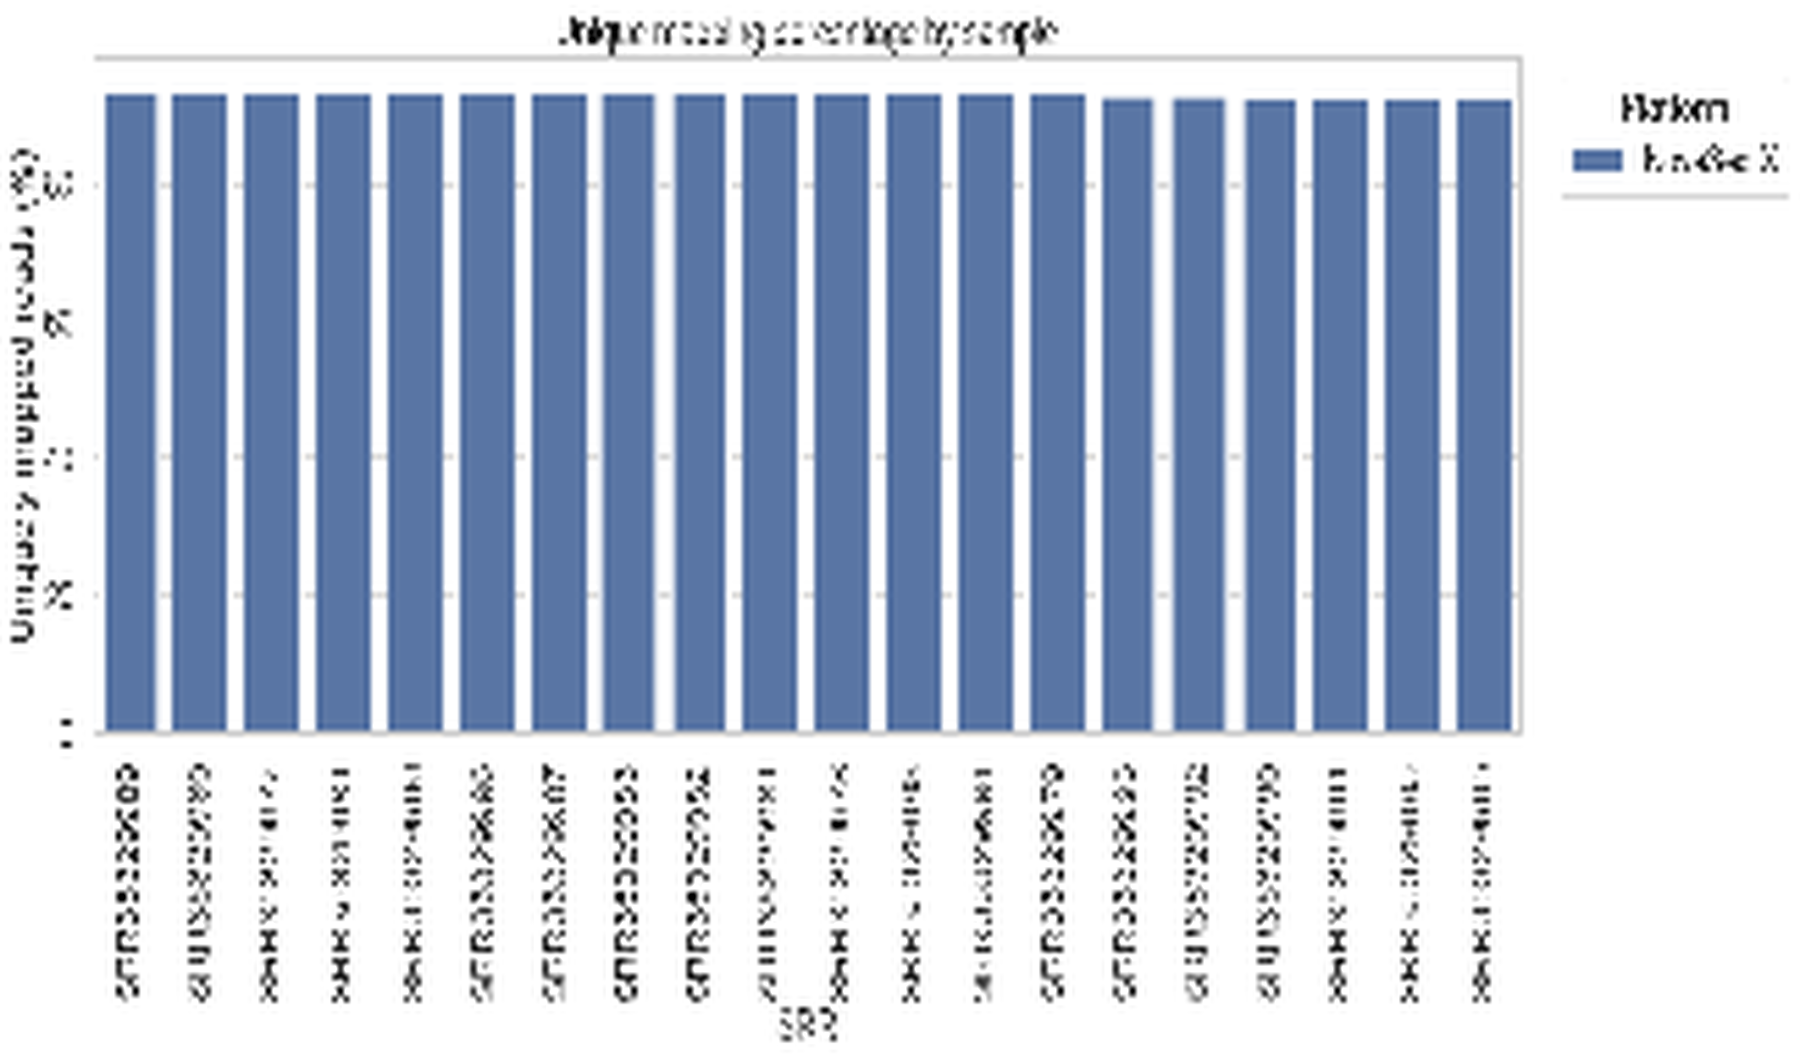
\includegraphics[width=\textwidth]{assets_htsa/alignment_unique_mapping_bar.png}
\end{minipage}\hfill
\begin{minipage}[t]{0.48\textwidth}
\centering
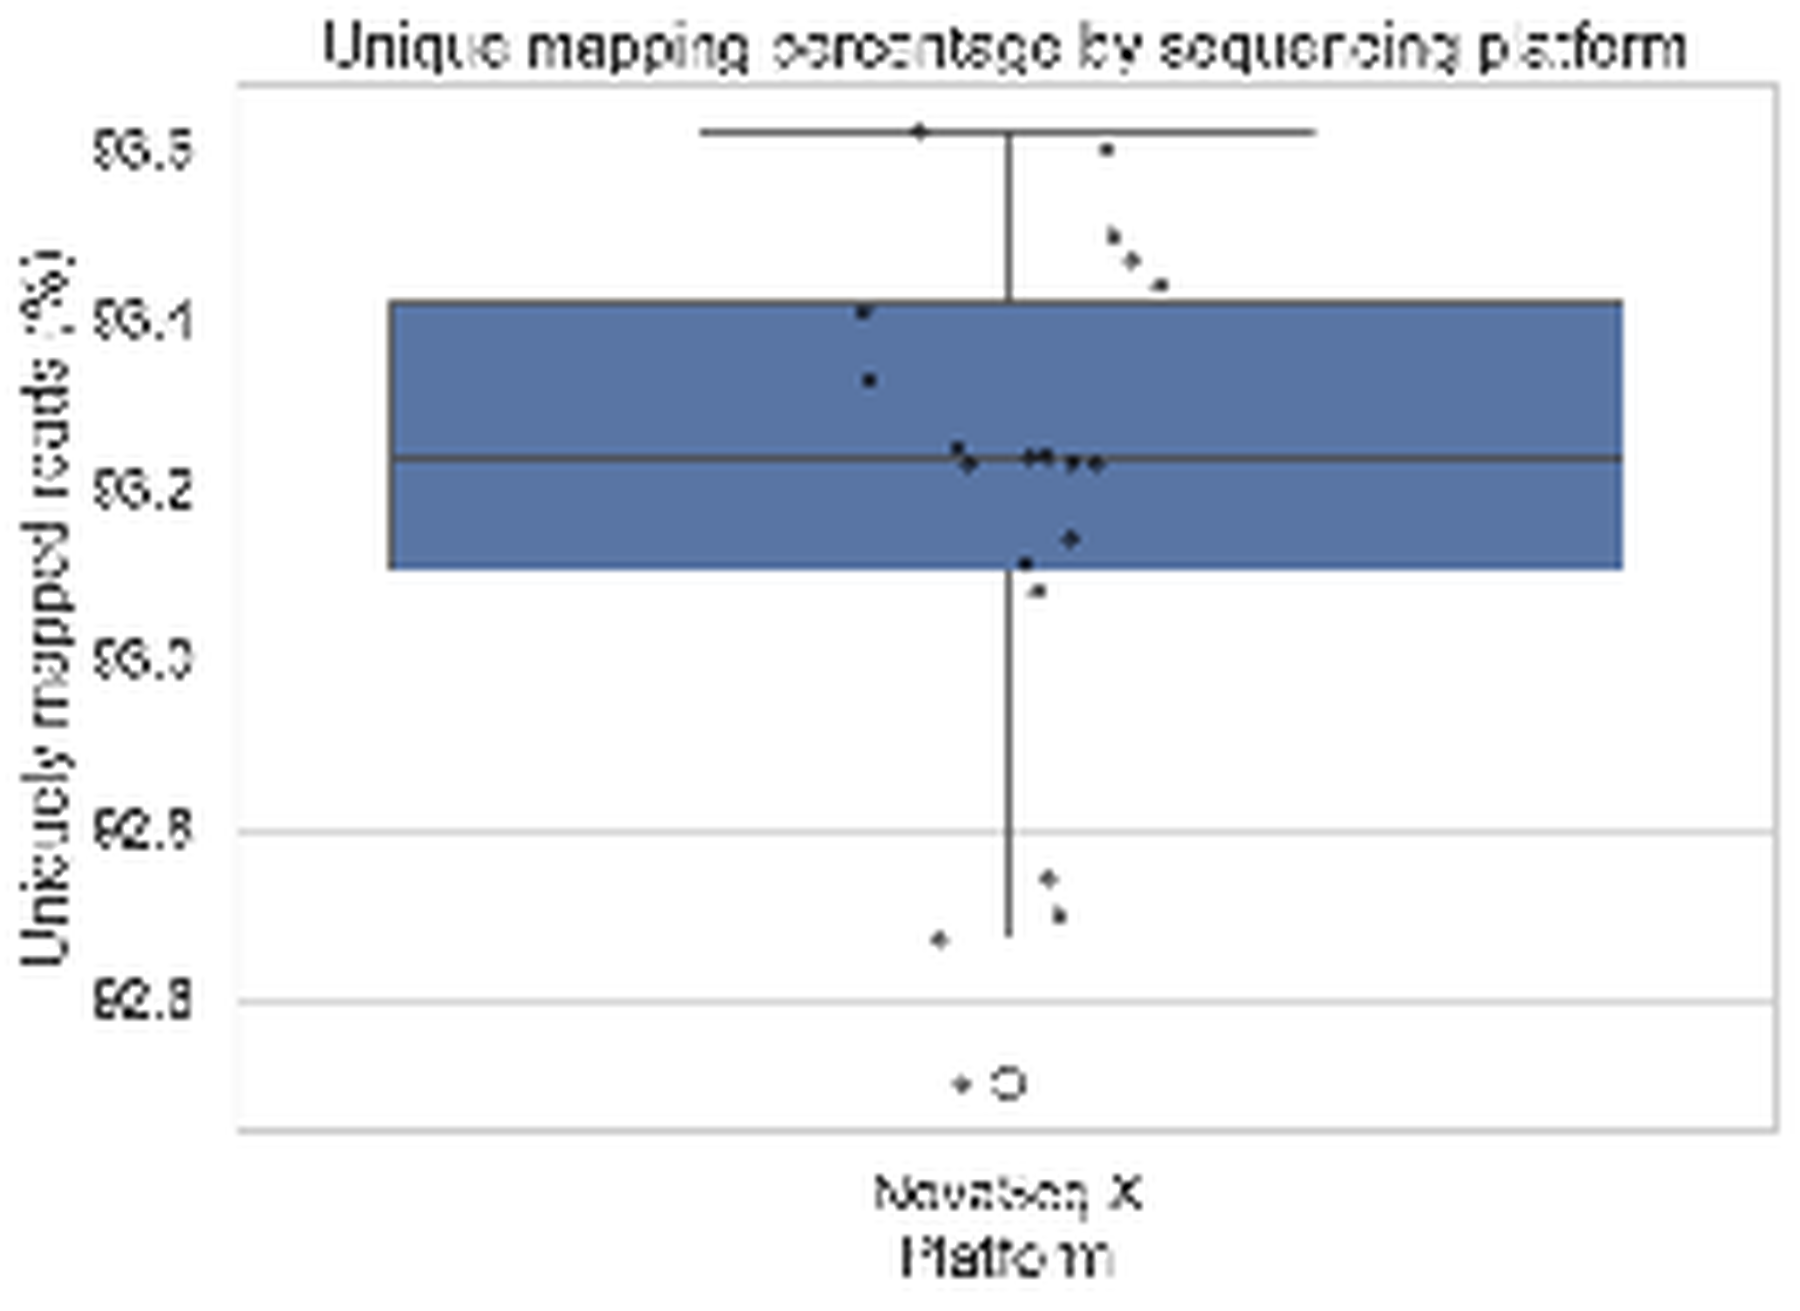
\includegraphics[width=\textwidth]{assets_htsa/alignment_unique_mapping_box.png}
\end{minipage}
\caption{Alignment statistics after mapping the trimmed reads to the GRCm39 \textit{Mus musculus} reference genome. Panel A shows uniquely mapped percentages for each sample, and Panel B shows the distribution of uniquely mapped reads across the full subset.}
\end{figure}

\begin{nikhipara}
Alignment of the trimmed reads to the GRCm39 reference genome produced consistently high mapping performance. Every sample exceeded 90\% uniquely mapped reads, with a median unique-mapping rate of 93.24\% and an interquartile range of 93.10--93.42\%. The lowest observed value was just below 92.6\%, but it remained within a high-quality alignment range relative to the rest of the cohort. These alignment metrics provided sufficient confidence to proceed with differential expression analysis.
\end{nikhipara}

\begin{piterpara}
Together, the QC and alignment checkpoints showed that the retained 20-sample subset was technically stable enough for downstream modeling. With the preprocessing concerns resolved, the next question became whether the biological structure of the dataset was driven more strongly by injury side or by genotype.
\end{piterpara}

\subsection{Differential Expression Analysis}

\begin{figure}[H]
\centering

\includegraphics[width=0.82\textwidth]{assets_htsa/results_pca.png}
\caption{Principal Component Analysis (PCA) of DRG transcriptomes. Samples are plotted along the first two principal components, which capture 46.2\% and 20.6\% of the variance, respectively. Shapes represent injury side and colors represent genotype.}
\end{figure}

\begin{sampara}
PCA was used to reduce the dimensionality of the dataset, which contained approximately 21{,}000 modeled genes across 20 mouse samples. The first two principal components captured 66.8\% of the variance. Samples separated more clearly by injury side (ipsilateral vs contralateral) than by genotype, with PC1 carrying the dominant side-associated structure and genotype contributing a weaker secondary pattern.
\end{sampara}

\begin{figure}[H]
\centering

\includegraphics[width=0.82\textwidth]{assets_htsa/results_sample_distance_heatmap.png}
\caption{Sample-to-sample distance heatmap of DRG transcriptomes. Euclidean distances were calculated from regularized log-transformed counts. Darker blue indicates higher similarity, and lighter blue indicates lower similarity.}
\end{figure}

\begin{sampara}
The sample-to-sample distance heatmap supported the same overall interpretation. Samples clustered primarily by injury side, with ipsilateral and contralateral samples forming the clearest separation in the matrix. Genotype still contributed structure within those broader groups, but it did not override the side-based organization. The agreement between the PCA and distance heatmap made side-specific contrasts the most defensible main path for follow-up analysis.
\end{sampara}

\begin{figure}[H]
\centering

\includegraphics[width=0.98\textwidth]{assets_htsa/results_bendpoint_volcano.png}
\caption{Comparison of volcano plots for the \artifact{ipsi\_vs\_contra\_in\_ff} contrast. Panel A shows the full significant set, and Panel B highlights the genes retained at the bend-point threshold.}
\end{figure}

\begin{nikhipara}
Because the side-specific contrasts produced very large sets of significant genes, a bend-point rule was used to reduce those outputs to more interpretable follow-up sets. In the \artifact{ipsi\_vs\_contra\_in\_ff} branch, the bend point occurred at an adjusted-\textit{p}-value threshold of \(1.37 \times 10^{-17}\), reducing the broader significant set to 709 genes. This narrowed subset still captured strongly supported differential expression while removing much of the dense background that made the full result harder to interpret biologically.
\end{nikhipara}

\clearpage
\subsection{Gene Ontology Analysis}

\begin{figure}[p]
\centering

\includegraphics[width=\textwidth,height=0.88\textheight,keepaspectratio]{assets_htsa/results_go_composite.png}
\caption{Gene Ontology (GO) analysis of the 709-gene \artifact{ipsi\_vs\_contra\_in\_ff} follow-up set. Biological Process, Cellular Component, and Molecular Function results are shown through lollipop plots and network views.}
\end{figure}

\begin{nikhipara}
Gene Ontology analysis was used to connect the 709-gene follow-up set to broader biological processes. Among the three GO categories, Biological Process provided the clearest and most coherent signal. The top enriched terms repeatedly pointed toward signaling and regulation, response to stimulus, morphogenesis, and stress-related remodeling, and the accompanying network view showed that many of those terms were connected through overlapping gene membership rather than representing isolated pathway stories.
\end{nikhipara}

\begin{nikhipara}
Cellular Component and Molecular Function results were more variable than Biological Process, but they still added context to the follow-up set. Cellular Component included more localized structural themes, while Molecular Function contained a smaller and less internally consistent set of enriched labels. Taken together, the GO results supported the view that the strongest FF branch signal was not just a list of highly significant genes, but a connected injury-response program that became easier to interpret after bend-point narrowing.
\end{nikhipara}

\clearpage
\section{Discussion}

\begin{piterpara}
\begin{piterpara}
The most robust finding in this dataset was that side-specific injury contrasts carried the strongest signal. Early QC and alignment checkpoints supported retaining this 20-sample DRG subset for downstream modeling, but the main interpretive shift came from the PCA-first review: side separated more clearly than genotype, while genotype behaved as a secondary axis with substantial overlap between paired WT and cKO samples. The PCA and sample-distance views converged on the same conclusion, making side-specific contrasts the most defensible primary path for interpretation.
\end{piterpara}

\begin{piterpara}
This PCA-first reading disciplined the interpretation of the differential-expression output. Rather than treating all modeled contrasts as equally informative, the workflow converged on a branch-priority logic in which \artifact{ipsi\_vs\_contra\_in\_ff} and \artifact{ipsi\_vs\_contra\_in\_cre} served as the main follow-up branches, while WT vs cKO in contralateral remained the strongest supporting genotype comparison. These secondary branches indicate that genotype effects are present, but they do not displace the side-specific injury signal as the dominant story.
\end{piterpara}

\begin{piterpara}
The bend-point step marked the transition from broad differential-expression output to a smaller and more interpretable follow-up set. For the two main side-specific contrasts, the ordered adjusted-\textit{p}-value curve reduced 7{,}023 and 7{,}541 significant genes to 709 and 870 genes, respectively. These smaller sets remained strongly supported statistically while becoming practical for pathway-level analysis. In that sense, the bend-point step made the most robust results easier to interpret against known injury and regeneration mechanisms.
\end{piterpara}

\begin{piterpara}
Among the follow-up branches, \artifact{ipsi\_vs\_contra\_in\_ff} remained the clearest pathway-level result. It combined a strong side-driven separation, a large but reducible differential-expression set, and the most coherent enrichment profile. Once shared-gene structure was examined through the chart, tree, and network views, the strongest upregulated terms converged around signaling, migration, morphogenesis, stress response, and neurogenic remodeling. That convergence made the WT branch the strongest biological centerpiece for the discussion and extended the original paper's candidate-gene logic into a broader transcriptomic context \parencite{halawani2023ahr}.
\end{piterpara}

\begin{piterpara}
These results still need to be read with caution. GO redundancy can make the functional signal look broader than it really is when overlapping labels are treated as independent findings, and the pathway summaries are persuasive only because they were interpreted after the PCA-first and bend-point-guided narrowing steps. Within those limits, however, the main discussion claim remains clear: this workflow converged on a robust side-specific injury-response program, and the WT branch provided the clearest pathway-level view of that response.
\end{piterpara}

\clearpage
\printbibliography

\end{document}
